%\documentclass[aps,prl,twocolumn,showpacs,superscriptaddress,groupedaddress]{revtex4}
%\documentclass[aps,showpacs,superscriptaddress,groupedaddress,preprint]{revtex4}
%\documentclass[prl,showpacs,superscriptaddress,groupedaddress,twocolumn]{revtex4}
%\documentclass[prl,showpacs,groupedaddress,twocolumn]{revtex4}
%\documentclass[twocolumn,superscriptaddress]{revtex4-1}
\documentclass[twocolumn,superscriptaddress]{revtex4-1}
%\usepackage{CJK}

%\usepackage{graphicx}  % needed for figures
\usepackage{bm}        % for math
\usepackage{amsfonts,amssymb,bbold,amsmath,amsthm,mathtools}% for math
\usepackage{mathrsfs}
%\usepackage[pdftex,letterpaper=true,pagebackref=false]{hyperref}
\usepackage{verbatim} %to use the \begin{comment} \end{comment}

\usepackage{hyperref}

\hyphenpenalty=2250

	\newtheorem{theorem}{Theorem}
	\newtheorem{lemma}[theorem]{Lemma}


\newtheorem{conjecture}[theorem]{Conjecture}
\newtheorem{corollary}[theorem]{Corollary}
\newtheorem{proposition}[theorem]{Proposition}
\newtheorem{fact}{Fact}[theorem]
\newtheorem{assumption}{N\!\!}

\theoremstyle{definition}
\newtheorem{definition}[theorem]{Definition}

\theoremstyle{remark}
\newtheorem{remark}[theorem]{Remark}

\newcommand{\bra}[1]{\langle#1|}
\newcommand{\ket}[1]{|#1\rangle}
\newcommand{\proj}[1]{| #1\rangle\!\langle #1 |}
\newcommand{\ketbra}[2]{|#1\rangle\!\langle#2|}
\newcommand{\braket}[2]{\langle#1|#2\rangle}

\newcommand{\bi}[2]{\binom{#1}{#2}}%{\begin{pmatrix} #1 \\  #2 \\ \end{pmatrix}   }
\DeclareMathOperator{\tr}{Tr}
\DeclareMathOperator{\sgn}{sgn}
\DeclareMathOperator{\vect}{vec}
\DeclareMathOperator{\sinc}{sinc}
\DeclareMathOperator{\mindist}{mindist}
\DeclareMathOperator{\wt}{wt}
\DeclareMathOperator{\tsum}{sum}
\DeclareMathOperator{\supp}{supp}
\DeclareMathOperator{\spann}{span}
\DeclareMathOperator{\card}{card}
\DeclareMathOperator{\SWAP}{SWAP}
%\DeclareMathOperator{\Pr}{Pr}

\def\Pr{{\rm Pr} }
\def\>{\rangle}
\def\rrangle{\rangle\!\rangle}
\def\<{\langle}
\def\llangle{\langle\!\langle}
\def\bk{{\bf k}}
\def\bx{{ \bf x}}
\def\by{{  \bf y}}


\def\bbA{\mathbb{A}}
\def\bbB{\mathbb{B}}
\def\bbC{\mathbb{C}}
\def\bbD{\mathbb{D}}
\def\bbE{\mathbb{E}}
\def\bbF{\mathbb{F}}
\def\bbG{\mathbb{G}}
\def\bbH{\mathbb{H}}
\def\bbI{\mathbb{I}}
\def\bbJ{\mathbb{J}}
\def\bbK{\mathbb{K}}
\def\bbL{\mathbb{L}}
\def\bbM{\mathbb{M}}
\def\bbN{\mathbb{N}}
\def\bbO{\mathbb{O}}
\def\bbP{\mathbb{P}}
\def\bbQ{\mathbb{Q}}
\def\bbR{\mathbb{R}}
\def\bbS{\mathbb{S}}
\def\bbT{\mathbb{T}}	
\def\bbU{\mathbb{U}}
\def\bbV{\mathbb{V}}
\def\bbW{\mathbb{W}}
\def\bbX{\mathbb{X}}
\def\bbY{\mathbb{Y}}
\def\bbZ{\mathbb{Z}}
\def\bbone{\mathbb{1}}

\def\cA{\mathcal{A}}
\def\cB{\mathcal{B}}
\def\cC{\mathcal{C}}
\def\cD{\mathcal{D}}
\def\cE{\mathcal{E}}
\def\cF{\mathcal{F}}
\def\cG{\mathcal{G}}
\def\cH{\mathcal{H}}
\def\cI{\mathcal{I}}
\def\cJ{\mathcal{J}}
\def\cK{\mathcal{K}}
\def\cL{\mathcal{L}}
\def\cM{\mathcal{M}}
\def\cN{\mathcal{N}}
\def\cP{\mathcal{P}}
\def\cQ{\mathcal{Q}}
\def\cR{\mathcal{R}}
\def\cS{\mathcal{S}}
\def\cT{\mathcal{T}}
\def\cU{\mathcal{U}}
\def\cV{\mathcal{V}}
\def\cX{\mathcal{X}}
\def\cY{\mathcal{Y}}
\def\cZ{\mathcal{Z}}

\def\rA{\rm{A}}
\def\rB{\rm{B}}
\def\rC{\rm{C}}
\def\rD{\rm{D}}
\def\rE{\rm{E}}
\def\rF{\rm{F}}
\def\rG{\rm{G}}
\def\rH{\rm{H}}
\def\rI{\rm{I}}
\def\rJ{\rm{J}}
\def\rK{\rm{K}}
\def\rL{\rm{L}}
\def\rM{\rm{M}}
\def\rN{\rm{N}}
\def\rP{\rm{P}}
\def\rQ{\rm{Q}}
\def\rR{\rm{R}}
\def\rS{\rm{S}}
\def\rT{\rm{T}}
\def\rU{\rm{U}}
\def\rV{\rm{V}}
\def\rX{\rm{X}}
\def\rY{\rm{Y}}
\def\rZ{\rm{Z}}

\def\ra{\rm{a}}
\def\rb{\rm{b}}
\def\rc{\rm{c}}
\def\rd{\rm{d}}
\def\re{\rm{e}}
\def\rf{\rm{f}}
\def\rg{\rm{g}}
\def\rh{\rm{h}}
\def\ri{\rm{i}}
\def\rj{\rm{j}}
\def\rk{\rm{k}}
\def\rl{\rm{l}}
\def\rn{\rm{n}}
\def\rp{\rm{p}}
\def\rr{\rm{r}}
\def\rs{\rm{s}}
\def\rt{{\rm t}}
\def\ru{{\rm u}}
\def\rv{{\rm v}}
\def\rx{{\rm x}}
\def\ry{{\rm y}}
\def\rz{{\rm z}}


\def\fB{\mathfrak{B}}
\def\fD{\mathfrak{D}}
\def\fF{\mathfrak{F}}
\def\fK{\mathfrak{K}}

\def\tA{{\bf{A}}}
\def\tB{{\bf{B}}}
\def\tC{{\bf{C}}}
\def\tD{{\bf{D}}}
\def\tE{{\bf{E}}}
\def\tF{{\bf{F}}}
\def\tG{{\bf{G}}}
\def\tH{{\bf{H}}}
\def\tI{{\bf{I}}}
\def\tJ{{\bf{J}}}
\def\tK{{\bf{K}}}
\def\tL{{\bf{L}}}
\def\tM{{\bf{M}}}
\def\tN{{\bf{N}}}
\def\tO{{\bf{O}}}
\def\tP{{\bf{P}}}
\def\tQ{{\bf{Q}}}
\def\tR{{\bf{R}}}
\def\tS{{\bf{S}}}
\def\tT{{\bf{T}}}	
\def\tU{{\bf{U}}}
\def\tV{{\bf{V}}}
\def\tW{{\bf{W}}}
\def\tX{{\bf{X}}}
\def\tY{{\bf{Y}}}
\def\tZ{{\bf{Z}}}



% Yingkai shortcuts
\def\del{\partial}
\def\XYZ{\{ {  X}, {  Y}, {  Z}  \}}

\def\floor#1{{\left \lfloor {#1} \right \rfloor  }}
\def\ceil#1{{\left  \lceil  {#1} \right \rceil   }}

\def\case#1{{\left\{  
	\begin{array}{ll}
  #1
	\end{array}
 \right.   }}
 
 
 
 
 \usepackage{multirow}
 \usepackage{circuitikz}
 \usepackage[]{mcode}


\usepackage{graphicx}
\usepackage{caption}
\usepackage{subcaption}



\begin{document}
%\begin{CJK*}{UTF8}{gbsn}

\title{Examining Brainwave Amplitudes in presence of External Audio Stimuli}%

\author{Joshua A. Kettlewell}
\affiliation{Singapore University of Technology and Design, 20 Dover Drive, Singapore 138682}
\author{Blake Perez}
\affiliation{Singapore University of Technology and Design, 20 Dover Drive, Singapore 138682}
\author{Giacomo Dalla Chiara}
\affiliation{Singapore University of Technology and Design, 20 Dover Drive, Singapore 138682}
\author{Thommen George Karimpanal}
\affiliation{Singapore University of Technology and Design, 20 Dover Drive, Singapore 138682}




\begin{abstract}
%\boldmath
We present a project report for course 30.502 (Research Methods), focusing on the effect of external auditory stimuli on various frequency components of brain waves using the \emph{Mindwave} EEG reader. We investigate to determine if there exists any statistically significant correlation between the amplitudes associated with certain brainwave frequencies and different types of auditory inputs. Our method uses the fast fourier transform to isolate relevant wavelength bands in order to compare the powers between different stimuli. We find that although there seems to be some degree of the above menioned correlation, it is not statistically significant. However, no conclusions can be drawn as the number of test subjects were limited, and the equipment used to measure brain waves may have had certain limitations which might have diminished the quality of our measurements.
\end{abstract}

\maketitle
%\end{CJK*}

\section{Introduction}
Brain waves or neural oscillations are rhythmic and repetitive electrical impulses generated by the neural activity in the central nervous system. The capturing and analysing of these signals is paramount to many fields such as neuroscience, cognitive psychology and cognitive linguistics to study several psychological and physiological phenomena. In a recent work \cite{asc} brain waves analysis has applied to study the acquisition of social interaction abilities in children with Autistic Spectrum Condition (ASC). Some of the symptoms of autism include general lack of social communication skills, including the inability to read body language, reduced interest in people and deficiencies to recognize emotions \cite{aut}, therefore increasing his/her chances of social isolation and depression. Although the limited social abilities, children with ASC are more emotionally responsive to a musical stimulus as compared to verbal or social ones. Hence, it may be possible use this musical stimulus to artificially develop and establish a map between pictures depicting various types of body language to their corresponding emotional states. \\
In another study by Giraldo and Ramirez \cite{activelistening} the authors explored the possibility to enrich auditory experiences using brain activity detection methods. By capturing the electrical signals generated by the brain and then mapping them to different emotional states, it is possible to alter several music parameters to enhance musical pleasure and certain emotions.\\
Following these experiments, we propose in Figure \ref{theory} a general framework for studying the relationship between music and brain waves. An individual is first exposed to a certain stimuli (musical or visual), and the resulting brain activity is capture, analysed and eventually mapped in real time to emotional states. Such information can then be used to control the stimuli.\\
As a first step in this direction, we try and investigate any statistically significant differences in the different frequency ranges of the brain waves when exposed to musical stimuli corresponding to different emotional states. In section \ref{teoria} we summarize the current models of musical emotions and the types of brain waves detected. In section \ref{exper} we then design an experiment for studying the possibility of efficiently capturing differences in brain waves generated by different audio stimuli. Finally, we describe the data collected, perform statistical analysis in section \ref{stat} and discuss the results in section \ref{concl}.

\begin{figure}[h!]
  \centering
      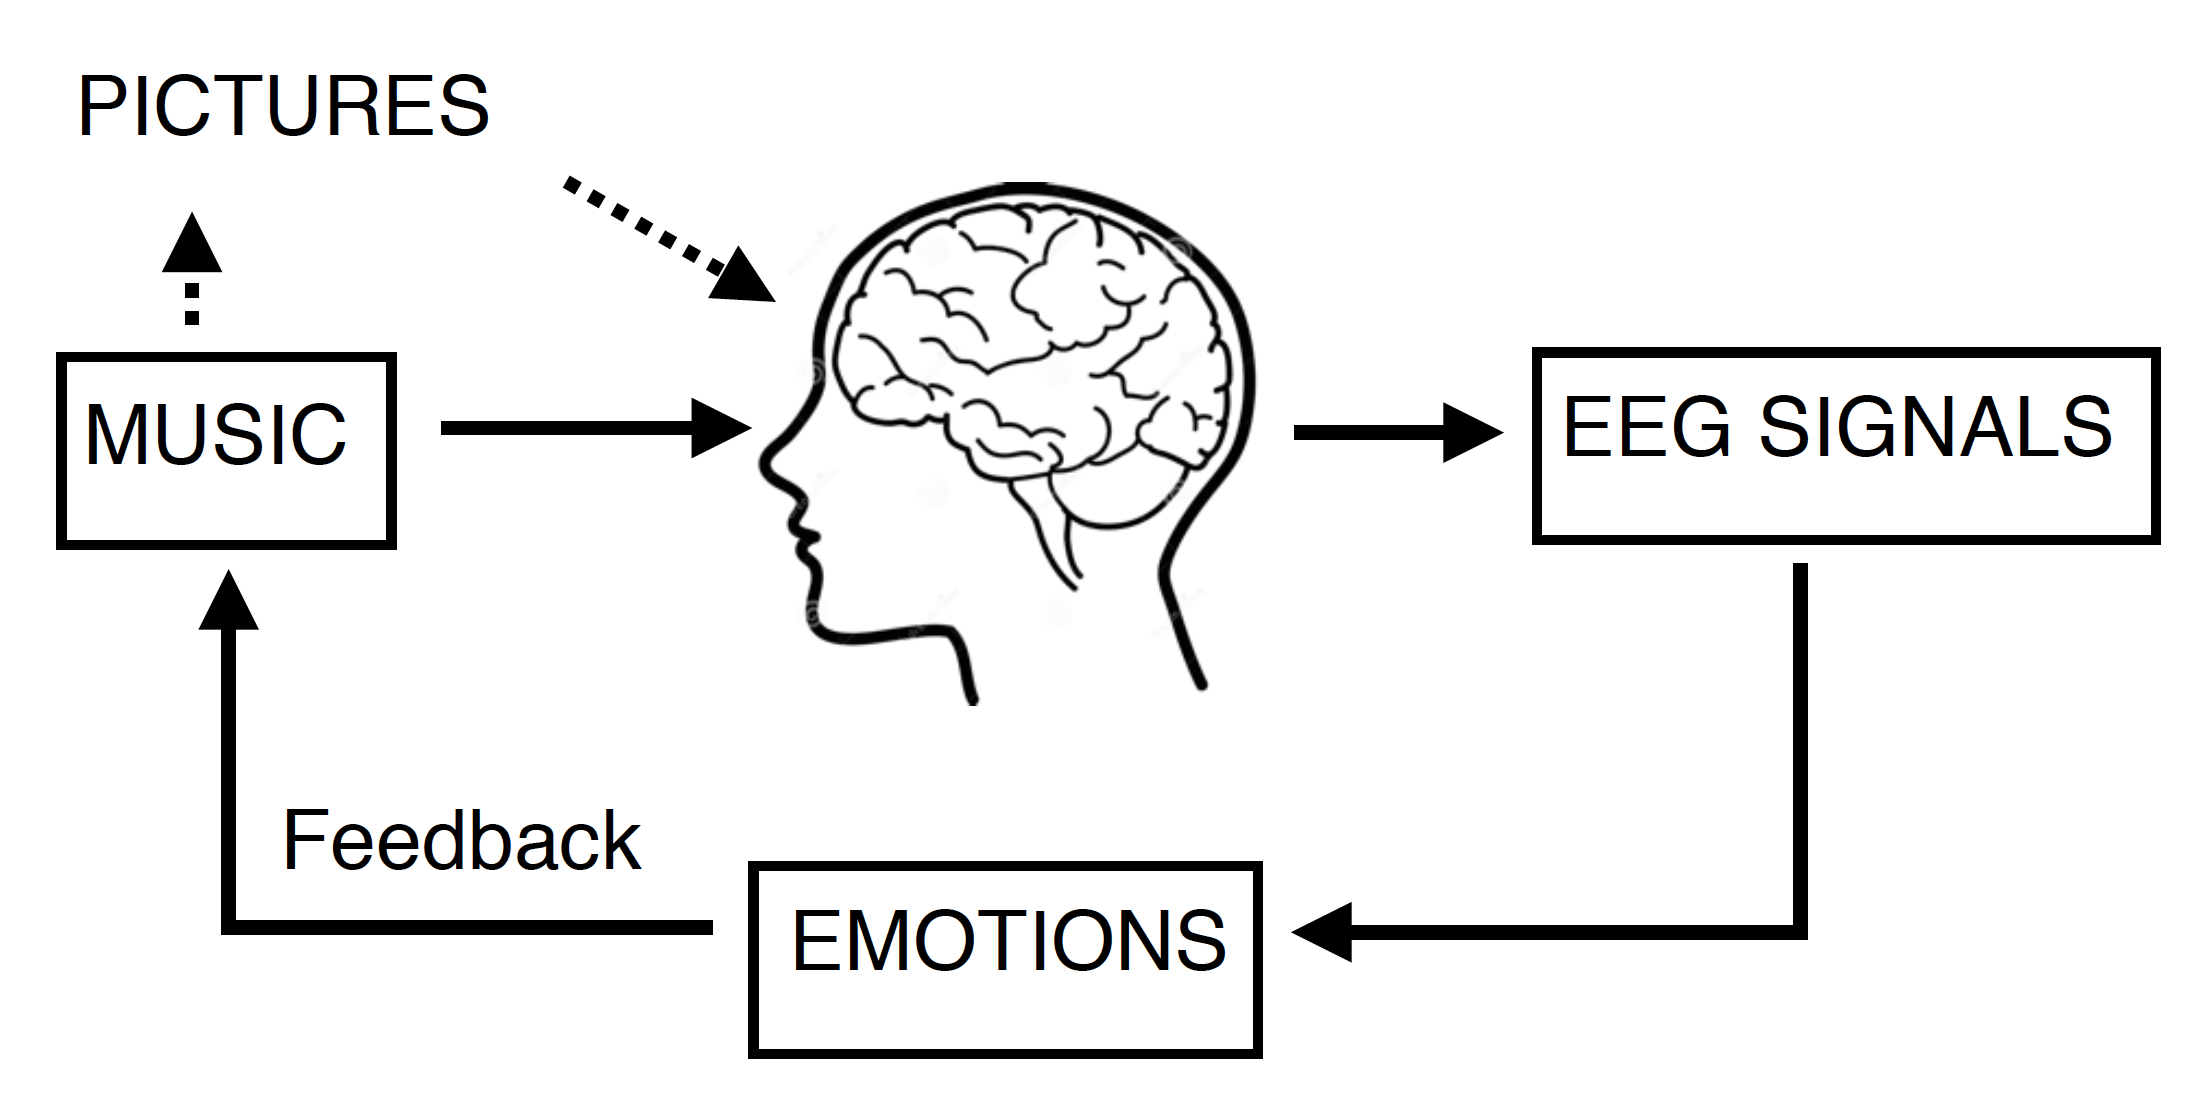
\includegraphics[width=0.4\textwidth]{figures/theory}
  \caption{\label{theory}  State-of-the-art framework for the study of music-brain interaction.}
\end{figure}






\section{Theoretical background} \label{teoria}%%%%%%%%%%%%%%%%%%%%%%%%%%%%%%
%%%%%%%%%%%%%%%%%%%%%%%%%%%%%%%%%%%%%%



\subsection{Models of musical emotions}

It has been proposed both by Russel\cite{musictype} and Thayer\cite{musictype2} that emotions can be  expressed on a 2 dimensional plane (\textit{dimensional models of emotions}), suggesting an interconnected neurophysical system is a conscious state. This is opposed to the \textit{discrete model of emotions} previously developed by Ekman \cite{ekman} and Panksepp \cite{pankssep} which states all emotions could be derived from different and independent neural systems. \\
Russel's dimensional model, with axis of \emph{valance} (pleasure-displeasure) and \emph{arousal} (activation-deactivation), is most commonly used  to measure participants emotional response to music, although Thayer's model, wherein the axis note \emph{energetic arousal} and \emph{tension arousal} is also utilised. It has previously been demonstrated that several music characteristics (\emph{i.e.} pitch, tempo and volume) may cause emotional responses \cite{juslin}, and both representations have been used to place songs in this emotional plane. In the current work we will made use of the Russel's emotional model (section \ref{exper}) in order to choose audio stimuli which should induce different emotions (i.e. emotions mapped in different quadrants of Russel's model). In the next section we provide a background on brain waves.

\begin{figure}[h!]
  \centering
      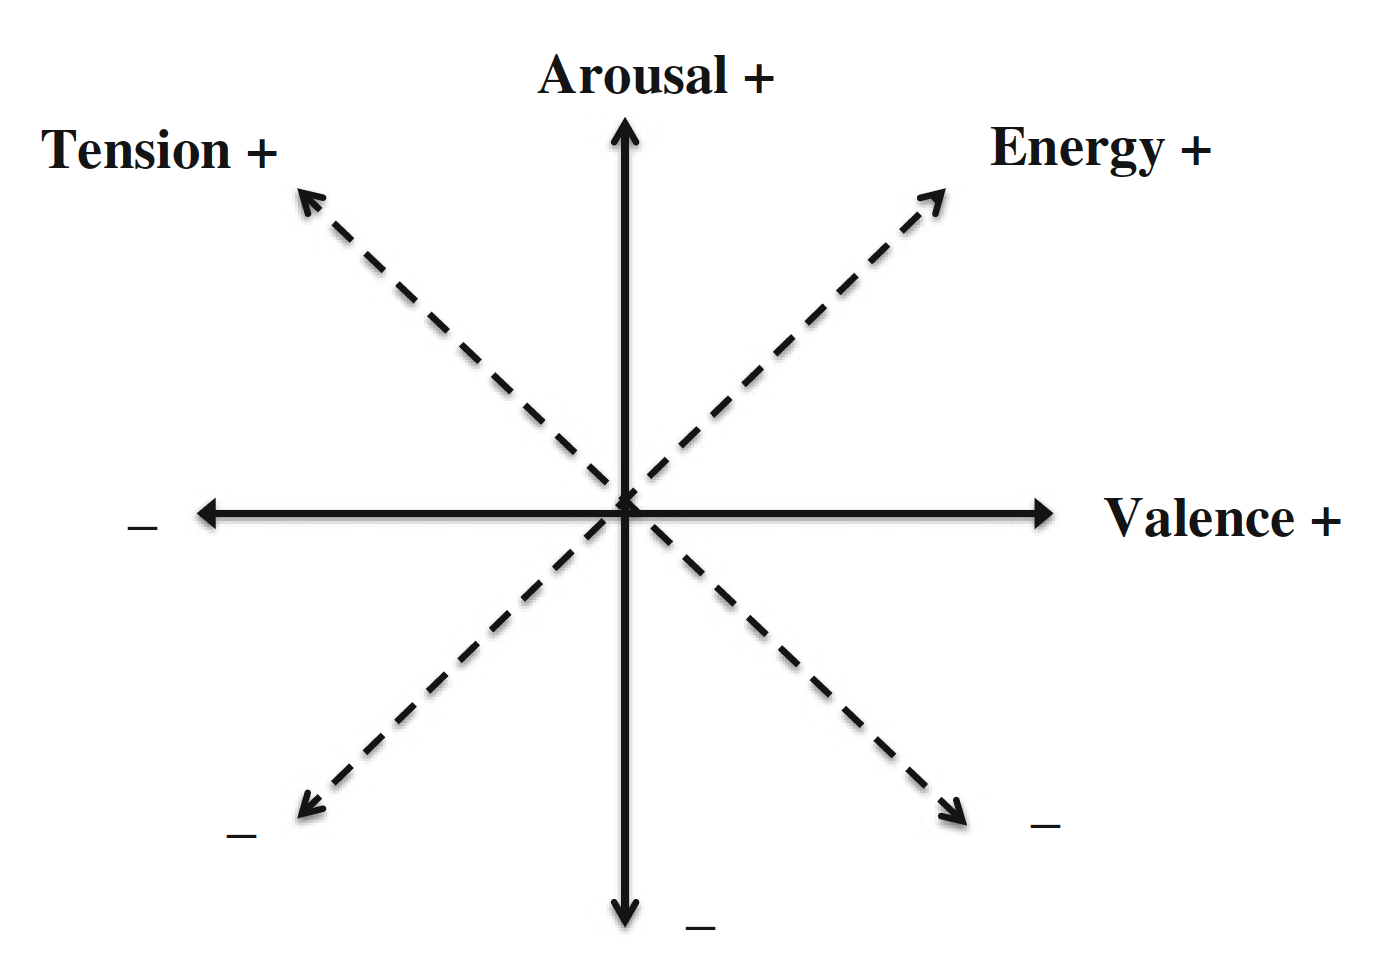
\includegraphics[width=0.35\textwidth]{figures/emotion_model}
  \caption{\label{emotion} Diagram of the dimensional emotion models: the dashed axis are used in the Thayer's dimensional emotion model, the solid axis are used proposed in Russell's circumplex dimensional emotion model \cite{book} }
\end{figure}



\subsection{Electroencephalography - EEG}

The brain is a network of many highly connected neurons which fire off electrical signals in order to communicate. If many fire at the same time then the induced change in electric potential may be measured from outside the skull. Brain waves are based on these electro-potential signal changes and are induced by different functions of the brain. These are entirely caused by firing neurons within the brain network with preforming various tasks, with different patterns relating to different behaviour. It has been long known that the average neuron firing patterns may oscillate at various frequencies - and that these frequencies in turn may be related to various states of consciousness. EEG readers record the changes in this electric potential and record the data electronically so the waveforms may be observed by outputting a serial stream of voltage measurements. \\
Although there are several methods for breaking the continuous frequency ranges of the brain into groups - we have followed the standard convention of breaking the complete signal into $5$ major groups. The frequency ranges examined in this report are as follows:

\begin{itemize}

\item  \textbf{Delta waves} \\
Delta waves occur in frequency range of $0-4 ~ Hz$. These tend to be the highest in amplitude recorded via EEG readers and are normally recorded throughout during infancy and in 'slow wave sleep' in adults. In adults they are primarily produced in the sub-cortical regions - near the front of the brain, although they are also found within the diffuse regions, and mid-line regions of the brain as well.

\item  \textbf{Theta waves} \\
Theta waves occur in frequency range of $4-7 ~ Hz$. These are usually associated with drowsiness in adults - however it may also be associated with meditation and states of intense creativity \cite{meditation}.They are also mostly associated with infancy and an excess of theta waves is associated with brain abnormality. \\

\item  \textbf{Alpha waves} \\
Alpha waves occur in the frequency range of $7-14 ~ H$. Primarily recorded in the posterior regions of the brain and typically higher in amplitude on the dominant side (associated in the side opposite to the dominant writing hand). Increases in amplitude are correlated with states of relaxation and the closing of the eyes. Attenuations in amplitude are correlated with either opening of the eyes or periods of mental fatigue.

\item  \textbf{Beta waves} \\
Beta waves occur in the frequency range of $14-30 ~ Hz$. These are produced primarily on the frontal regions of the brain and distributed evenly between both hemispheres. Generally these are associated with muscular movement orders and to a lesser extend periods of active concentration \cite{beta}. Absence or lower amplitude beta waves are correlated with cortical damage and periodic changes in amplitude may be caused by various benzodiazepines and halluionogentics. Beta waves are the found to be the dominant waves in patients who have their eyes open or are nervous. \\

\item  \textbf{Gamma waves} \\
Gamma waves occur on the frequency range of $30-100 ~ Hz$. These are associated with the linking signals between collective bunches on neurons to perform motor or cognitive functions \cite{basics}.

\end{itemize}










\section{Experimental set up}  \label{exper}%%%%%%%%%%%%%%%%%%%%%%%%%%%%%%%%%%%%%%


\begin{center}
\textbf{Song choice}
\end{center} 

As we wish to compare collected brainwaves between varying audio stimuli, songs with a large hypothetical difference in emotional response are selected. Russel’s circumplex model [3] is used. The circumplex model splits common mood descriptions over a 2D plane with the axis of \emph{Arousal} and \emph{Valence}. Jaimovich \emph{et al.} previously applied textually derived emotional responses to different songs from survey responses and ranked them according to the circumplex model \cite{musictype}. Using this emotional assignment of songs, we selected songs with a large separation in emotional space; ”Hallelujah - Jeff Buckley” and ”Smells like teen spirit - Nirvana”. The songs lie in the first and third quadrant of the model respectively.

\begin{figure}[h!]
  \centering
      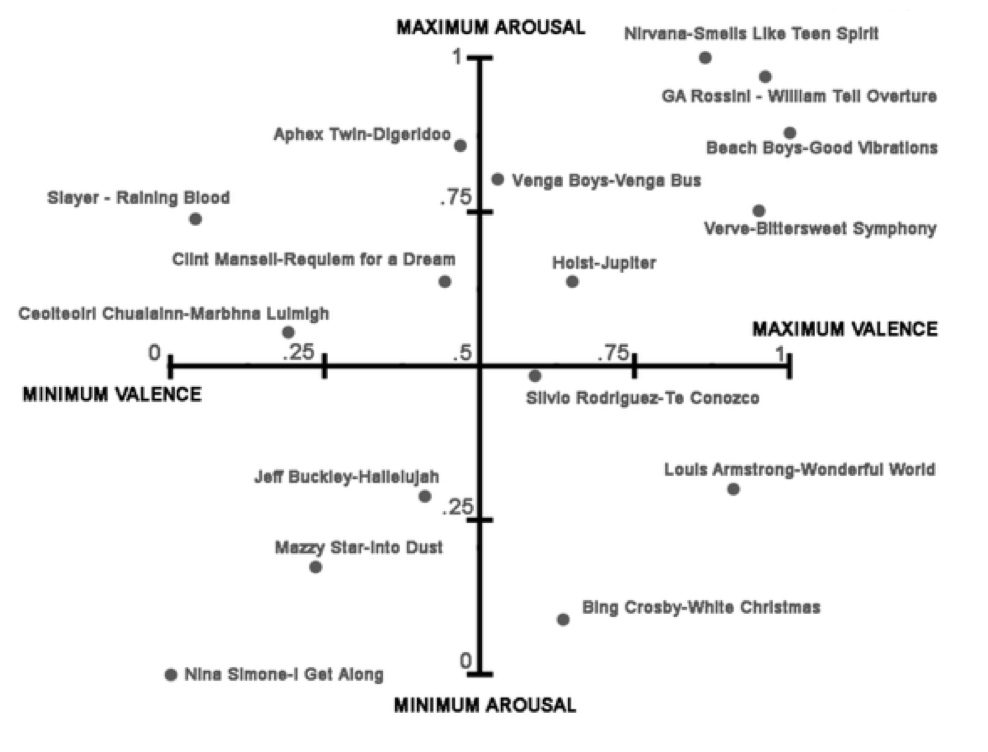
\includegraphics[width=0.5\textwidth]{song_choice}
  \caption{A popular ranking system showing how a variety of songs score for arousal an valence.}
\end{figure}

One-minute samples are taken from each of these tracks and separated with white noise to create one complete track. Code was prepared to sync the EEG reader with the track so recording would begin with the track and end 10 seconds after completion in case there was in lag in the track’s initialization - allowing all of the data to be used without a need to cut any parts away. 

\begin{figure}[h!]
  \centering
      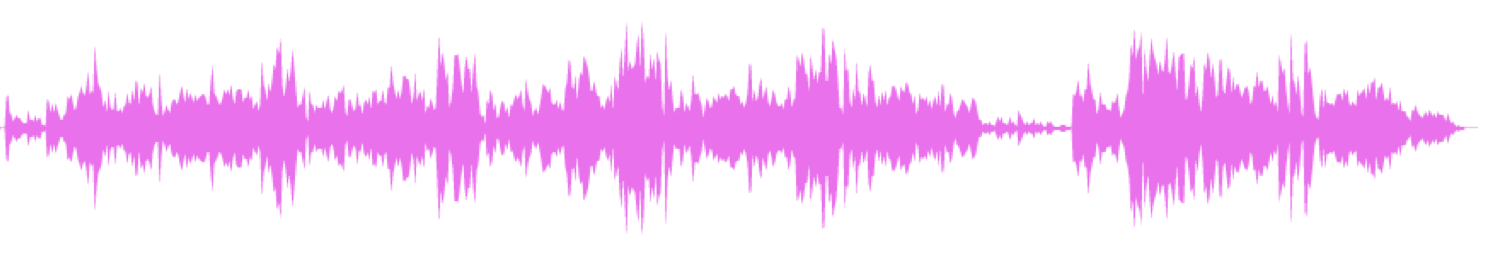
\includegraphics[width=0.5\textwidth]{jeffbuckley}
  \caption{The time dependent sound intensity of "Hallelujah", The initial period of low intensity was used for the experiment.}
\end{figure}

\begin{figure}[h!]
  \centering
      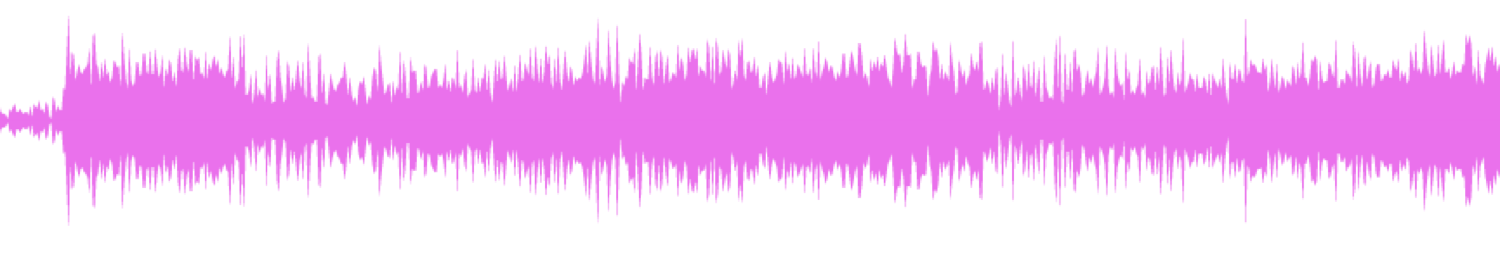
\includegraphics[width=0.5\textwidth]{nirvana}
  \caption{The time dependent sound intensity of "Smells like teen spirit",  a section for the center of the track was sampled for the experiment due to featuring of the chorus and to avoid a quieter introductory section.}
\end{figure}


\begin{center}
\textbf{EEG Details}
\end{center} 

\emph{Mindwave} is a low budget Electroencephalography (EEG) and requires minimal calibration and setup. The device connects wirelessly via bluetooth link to a single computer. The mindwave uses its own bluetooth adapter that transmits and receives signals. Custom code provided by Chen Lujie parses the raw data into a single vector of signal power data that is outputted to a .CSV file.

The \emph{mindwave} is unique from most EEG devices largely because of its low cost. However, the unit does have some limitations. Unlike most commercial EEG units, the \emph{Mindwave} has only one sensor that is located at the center of the forehead. Literature suggests that different brainwave spectrum may be stronger or more present in different areas of the brain. Thereby it is expected that the unit will be most sensitive to delta waves as they occur in the frontal lobes of the brain. Signals from the other waves may be more difficult to measure as they propagate from spatially distant localities. 

\begin{figure}[h!]
  \centering
      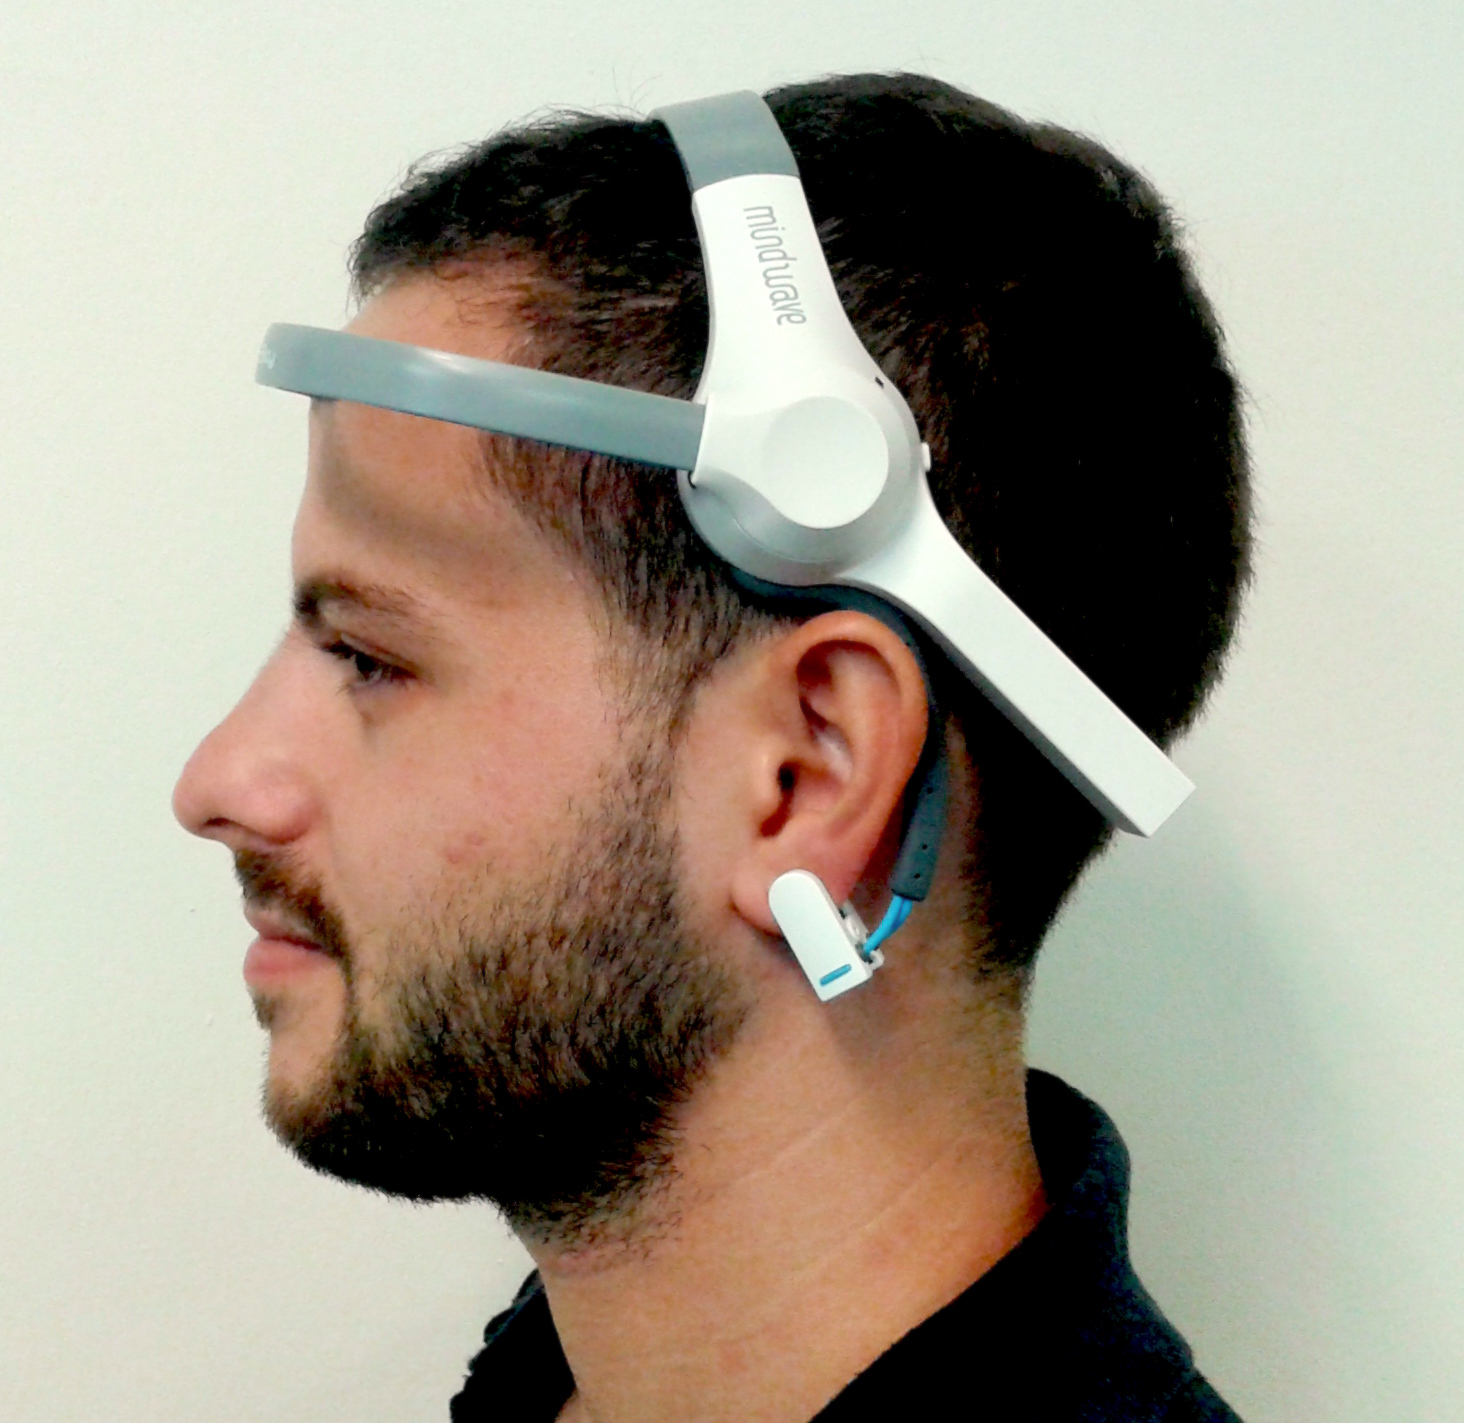
\includegraphics[width=0.3\textwidth]{figures/zakside1}
  \caption{A participant wearing the EEG reader. A frontal electrodiode in contact with the forehead records electrical potential changes.}
\end{figure}


An experiment is constructed to ascertain whether auditory stimuli can have a measurable effect on participant's brainwaves. Measurable is defined as being statistically discernible from the \emph{Mindwave} EEG reader data. Our hypothesis is as follows.

\textbf{Hypothesis:}
Auditory stimuli associated with different feelings of arousal can produce a noticeable change in the emergence of different brain wave amplitudes across a broad range of participants.\\

This project focuses on the results of a single experiment with nine trials. The protocol is as follows:

\begin{itemize}
\item Experiment 1
\begin{enumerate}
\item A participant is placed in a quiet room with no external auditory stimuli. The \emph{mindwave} EEG reader is fitted. The participant is informed that he or she will be listening to three audio tracks in succession. They are then instructed to rest their hands on the desk and close their eyes to mitigate noise from blinking or movement.
\item Jeff Buckley’s \emph{Hallelujah} is played while the subject remains motionless. This continues for 60 seconds. 
\item White noise is played for 60 more seconds. 
\item Nirvana’s \emph{Smells Like Teen Spirit} is then played for 60 seconds. 
\item This experiment is repeated for several participants. Data is split into the various components relating to different tracks. 
\item Power of the brainwave bandwidths is then compared between different auditory inputs. 

\end{enumerate}
\end{itemize}

The long periods of music were chosen to both ensure that the participants had time to adjust to the different audio stimuli and that brainwaves in low frequencies would be recorded. It was also hoped that this would reduce the effect of noise on the total sample. The segmentation and filtering of the data is discussed in the following section. 







%%%%%%%%%%%%%%%%%%%%%%%%%%%%%%%%%%%%%%%%%%%%%%%%%%%%%%%%%%%%%%%%%
\section{Data analysis}  \label{stat}%%%%%%%%%%%%%%%%%%%%%%%%%%%%%%%%%%%%%%%%%%%%%%%%

In the current section we will first describe the \textit{raw data} (EEG) collected during the experiment, and the preliminary treatment of outliers. We then decompose the original signals into its frequency components using the Fast Fourier Transform algorithm and identify the presence of the different wave forms. We conclude performing statistical hypothesis testing. The MATLAB code for processing the raw data is included in the appendix. \\


\subsection{Data collected}

The experiment has been performed on 9 volunteers (adults), from whom EEG data has been recorded. In Figure \ref{datata} we plot the original EEG signals from 8 subjects studied (data collected on one of the 9 participants has been excluded). Preliminary examination of the raw data reveals that there exists three clusters of subjects, namely, those corresponding to relatively clean data, with certain apparent patterns clearly visible, those with clean data with some sections of apparent noise, and those with very noisy data. It may be the case that in participants whose data was significantly noisy, the electrodes of the EEG may not have been in good contact with the skin. \\
Following data collection, it was found that despite the data collection being taken over an equal time period for all participants, a different number of data points were recorded.  In order to handle this anomaly, it was assumed that the EEG sensor being used recorded samples at different sampling rates during different recordings. The collected data was scaled accordingly.\\
Certain noticeable outliers were also manually removed prior to data analysis. Also, data from one of the participants was excluded due to the presence of large amount of noise in the recordings. The source of this noise was concluded to have arisen from the facial movements that were observed during data collection on this participant.\\
 
\begin{figure}[h!]
  \centering     
   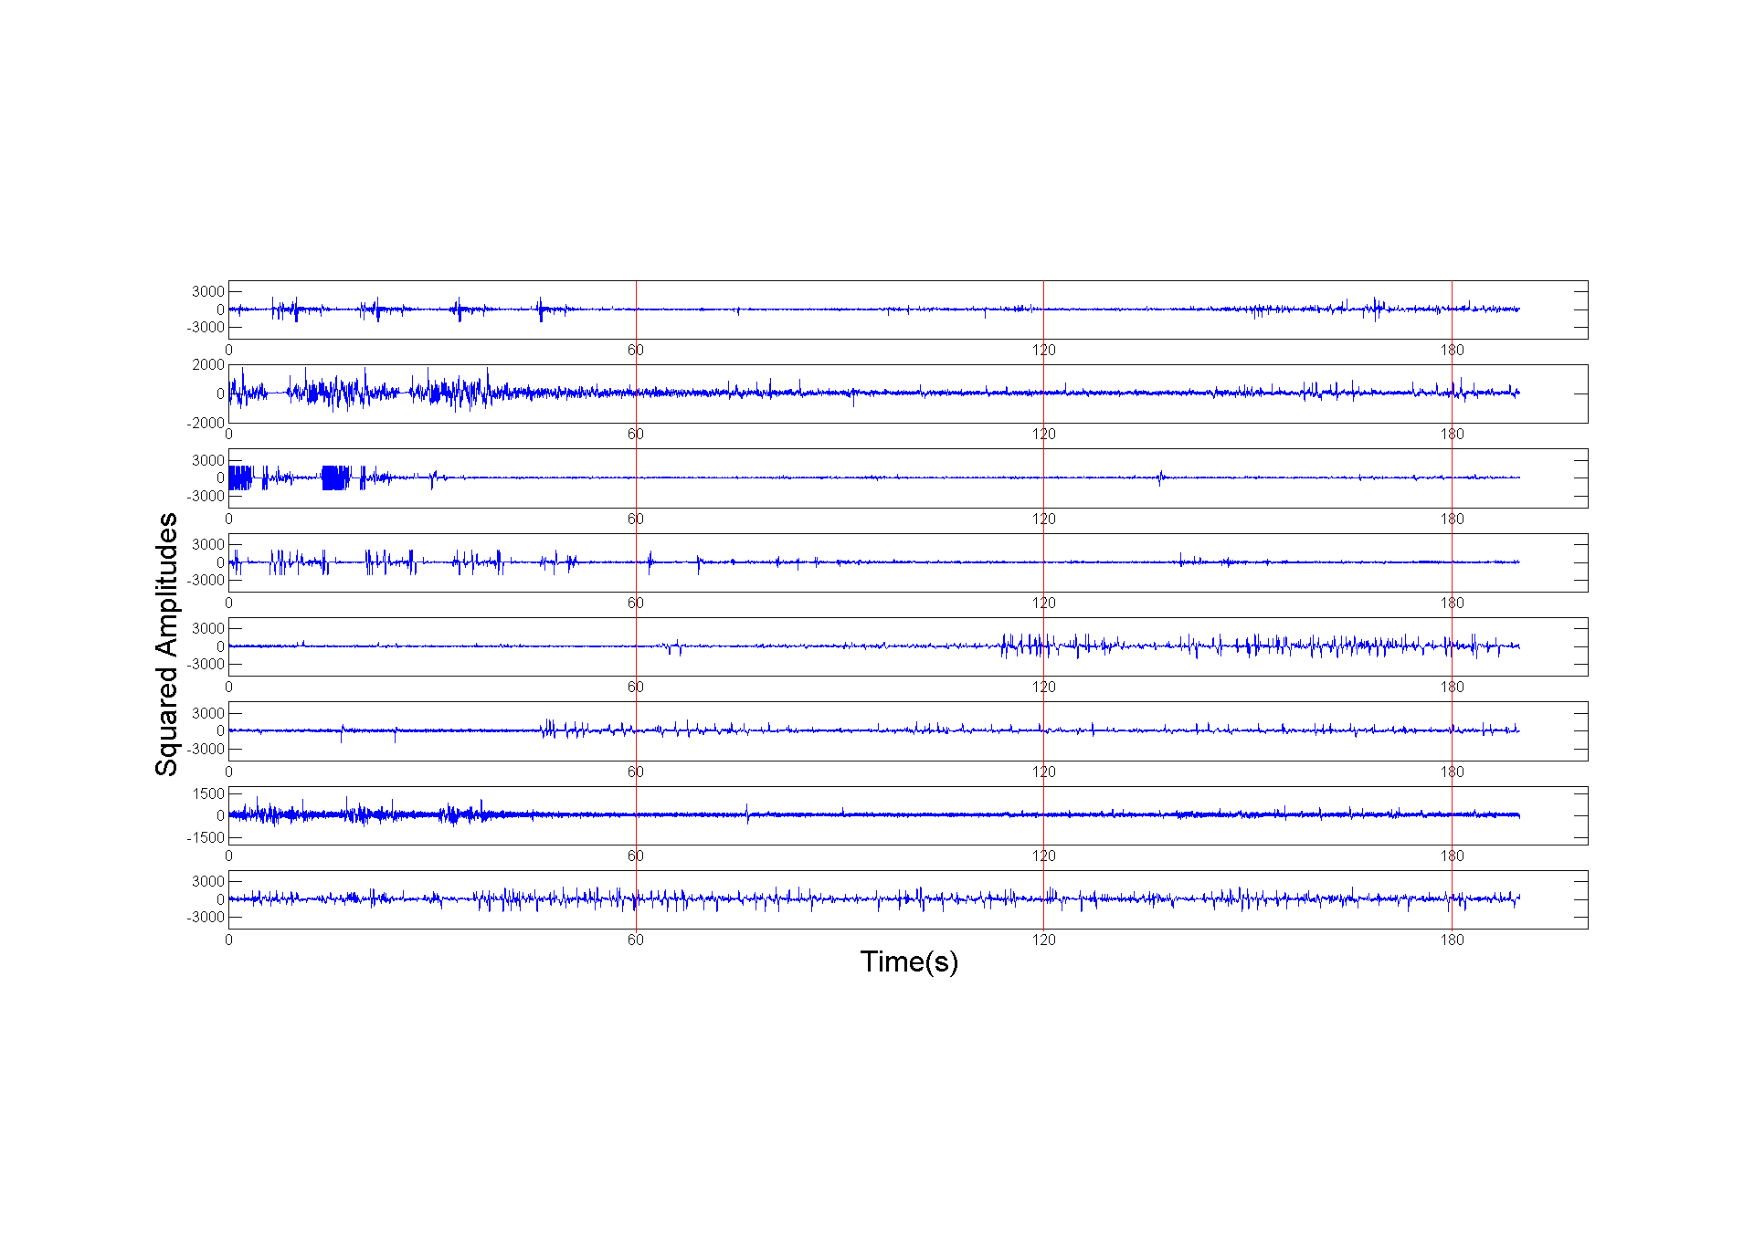
\includegraphics[width=0.55\textwidth]{all_waves}
  \caption{\label{datata}The complete set of all 8 recordings used for data analysis. A single data set was eliminated from the set due to high amount of noise present. There initially appears to be some correlation between signal intensity in different ranges.}
\end{figure}



\subsection{Fourier Transform and Waveband power isolation}

In order to transform the raw time varying sensor data into the frequency domain, the Fast Fourier Transform (FFT) algorithm was used. The FFT of a signal x is defined as indicated below:
\begin{align}
X_k\ \stackrel{\text{def}}{=}\ \sum_{n=0}^{N-1} x_n \cdot e^{-i 2 \pi k n / N},  \quad k\in\mathbb{Z}\,
\end{align}

The raw time series data was divided into three parts, each corresponding to a particular type of sound (song A, white noise or song B), and each lasting for 60 seconds. The FFT was perfored on each of these parts separately to reveal the relative squared amplitudes or powers corresponding to each frequency.  Due to some inconsistencies in the sampling time of the sensor, it was assumed that the sensors transmit at a constant rate throughout a particular recording. In order to incorporate the above mentioned assumption, a scaling factor was used to scale the horizontal axis of the time series data according to its sampling rate. Also, since the actual time duration of each part in a particular recording was 60 seconds, the horizontal axis of the frequency spectrum had to be scaled by a factor of 60 in order to obtain the true frequencies on the horizontal axis. \\
Once the frequency spectrum of each part was obtained, the frequencies were binned into delta, theta, alpha, beta and gamma wave frequency bands based on neuroscience literature \cite{thommen}. Figure \ref{bins} shows the cut-off frequencies for each band is shown below:     

     \begin{figure}[h!]
  \centering
      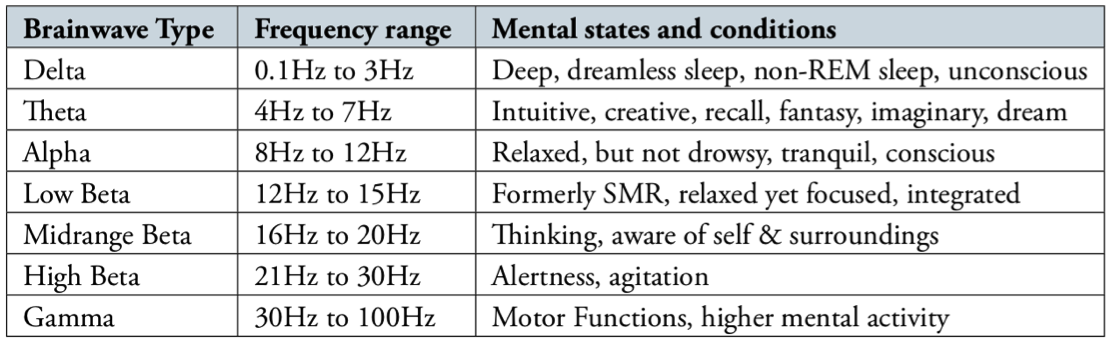
\includegraphics[width=0.5\textwidth]{brainwavespic.png}
  \caption{\label{bins} Table showing the frequency bins used in the data processing.}
  \label{wavecomp}
\end{figure}

The power associated with each frequency band was then determined by integrating the discrete power values within that particular band. Later on, these integrated power values were compared using a Wilcoxon test in order to determine whether there is any statistically significant difference between them for different types of sounds. Following the Fourier Transform procedure, amplitudes of the different wave bands could be contrasted between different audio stimuli.   \\

\begin{figure}[h!]
  \centering
      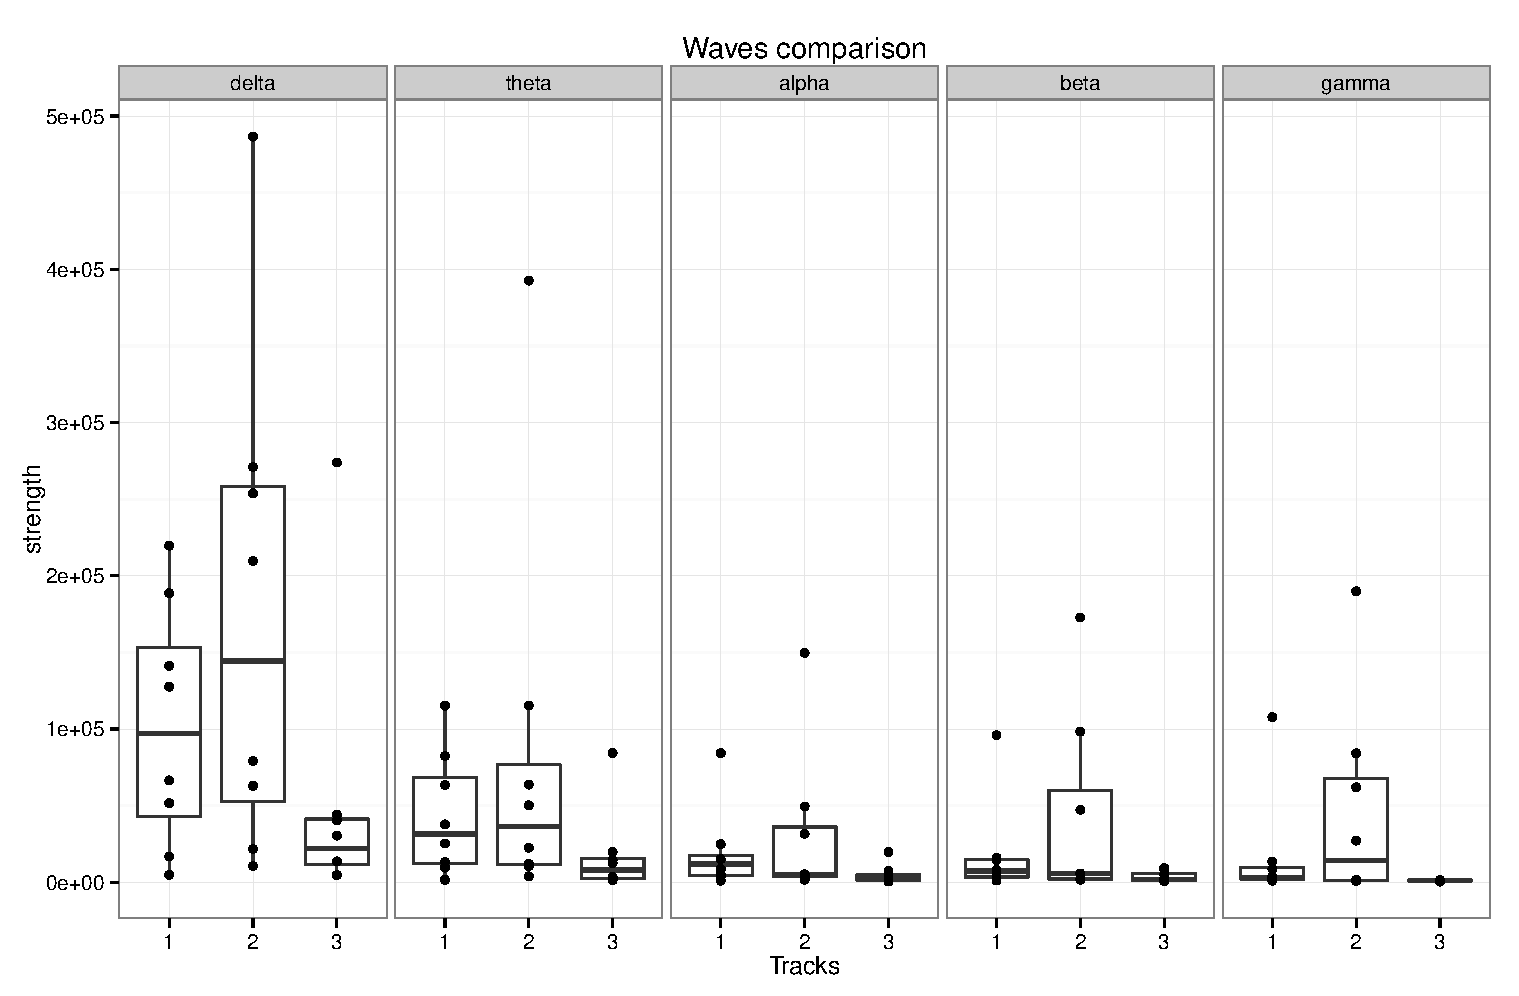
\includegraphics[width=0.5\textwidth]{compare_waves}
  \caption{Boxplot showing the comparisons across each wave band across all audio stimuli. \emph{R-statistics} was utilised to produce the box plot - bar indicate median, box edges for $\pm 25$ percentiles and lines to $\pm 50$ percentiles. Points outside 1.5 times the $25-75$ percentile range were taken to be anomalous. Each point shows data from a single participant.}
  \label{wavecomp}
\end{figure}

In Figure \ref{wavecomp} we compare the power values for each particular frequency range across the participants and across the different audio stimuli. On the y-axis are reported the value of the powers, while the top and bottom horizontal axis report the different categories over which the power has been measured (audio stimuli and frequency range). The boxes indicate the first, second (median) and third quartiles of the data observed. Vertical lines spans until the maximum and minimum observed values, while an isolated point might be considerate as a potential outlier ($1.5$ standard deviation further form the median). \\
Firstly, we observe that the amplitude of the low frequency waves is significantly high as compared to other frequencies. A potential explanation for this observation is that the low frequency delta waves are known to be both of the highest amplitude and are also most prominent in the pre-frontal cortex in adults - which included the entirety of the participants  (the EEG used is comprised only of a single sensor placed upon the forehead of the participant). \\
Interestingly, the results do seem to show an increase in the amplitudes across \emph{all} frequency bands when the white noise is played between the two musical tracks. Although this was not expected, it may be that brain activity during this intermediate period of white noise is associated with deep thought (the participants were instructed to sit in silence without movement - in a meditation like state.). This was not initially considered by the authors however, the increase of brainwave amplitudes in when audio stimuli is removed is a point of interest. \\
 

\subsection{Wilcoxon test}
In order to test for the difference in mean intensity of the delta waves induced by the first song, the second song and the white noise, we design the hypothesis testing and run them using the Wilcoxon test. In particular, we wish to test the following three hypotheses, where $\mu_1, \mu_2, \mu_{wn}$ are respectively the mean intensity of the delta waves generated during the first song, the second song and the white noise:

\begin{align}
\label{f1}
H_0: \quad \mu_1 = \mu_2 , \qquad H_1: \quad \mu_1 \neq \mu_2
\end{align}
\begin{align}
\label{f2}
H_0: \quad \mu_1 = \mu_{wn} , \qquad H_1: \quad \mu_1 \neq \mu_{wn}
\end{align}
\begin{align}
\label{f3}
H_0: \quad \mu_2 = \mu_{wn} , \qquad H_1: \quad \mu_2 \neq \mu_{wn}
\end{align}

The Wilcoxon test is a non-parametric statistical test for paired samples (the samples collected are \textit{paired} since EEG data is collected on the same subject for different musical stimulus). The choice of a non-parametric test  is justified by the small sample size, for which normal distribution of the underlying population cannot be assumed. The Wilcox test pool together the two samples considered (of size $n$ and $m$)  and compute for each observed value its respective rank. For $Z_i, i=1...n$ being the observed value from the first sample, and for $Z_{n+j}, j=1,...m$ being the observed values from the second sample, we compute the respective ranks $Ri := rank(Z_i)$. The test statistic is then:
\begin{align}
T^{Wilcoxon} = \sum_i^{n} R_i
\end{align}
Large values of $T^{Wilcoxon}$ mean that the observed value of the first group are generally larger than the ones from the second group , and hence indicate evidence against $H_0$. For a treatment of the Wilcoxon test theory we refer to \cite{sara}. We have used the R function \textit{wilcoxon.test} (see appendix).\\

In the following table we report the respective p-values for the three tests described in \ref{f1} ,  \ref{f2} and \ref{f3}. 
\\
\vspace{10pt}

\begin{tabular}{ l | l  }
Songs Compared & P values \\ \hline
  Song A, Song B	& 0.2969 \\
  Song A, White Noise & 0.07813\\
  Song B, White Noise & 0.4688
\end{tabular}







%%%%%%%%%%%%%%%%%%%%%%%%%%%%%%%%%%%%%%%%%%%%%%%%%%%%%%%%%%%%%%%%%
\section{Concluding remarks} \label{concl}%%%%%%%%%%%%%%%%%%%%%%%%%%%%%%%%%%%%%%%%%%%

In this work, a general framework for the study of the relationship between music and brain activity has been proposed, and a procedure to collect neural oscillations induced by audio stimuli was described. In addition, several drawbacks of the sensor, including its variable sampling time and its bias for delta wave frequencies was mentioned. The methods for taking these inconsistencies into consideration and for removing outliers before transforming the data into its frequency domain was also explained. The bias towards delta wave frequencies was confirmed by their significantly larger squared amplitudes in the frequency spectrum. Based on established guidelines of binning different frequency components, the strength of the different frequency components of the brain waves was obtained. Finally, the transformed data was analysed using the statistical non-parametric Wilcoxon test in order to determine the existence of any significant differences in the strengths of the delta frequency components for the different types of sounds. It was found that although certain patterns could be observed from the raw data qualitatively, the high p-values obtained from the Wilcoxon test on the transformed were too large to conclude the existence of any statistically significant differences between the different sounds.   
This however, may not imply the non existence of any considerable differences in the transformed data, as it can be observed in the plot of the raw signals. It must be acknowledged that the sensor used for data collection had certain limitations, and the sample size was too small to arrive at any conclusions. \\






\begin{thebibliography}{}

\bibitem{asc} Acquisition of social abilities through musical tangible user interface: children with autism spectrum  condition and the reactable, Lila Villafuarte, Sergi Jorda, Milena Markova, CHI 2012
\bibitem{emotion} Emotion in Motion:
A Study of Music and Affective Response, Javier Jaimovich, Niall Coghlan and R. Benjamin Knapp

\bibitem{activelistening} Brain activity driven by real time music emotive control, Sergio Giraldo, Rafael Ramirez, BCI Meeting 2013

\bibitem{musictype} A Circumplex Model of Affect, James A Russel, Journal of Personality and Social pycology, 1980, 

\bibitem{musictype2} Thayer J, Faith M (2001), A dynami systems model of musically induced emotions. Ann N Y Acad Sci (((1):452-456

\bibitem{ekman} Ekman P 1992, An arguement for basic emotions, Cogn Emot 6(3-4):169-200

\bibitem{pankssep} Pankssep 1992, A Critical role for "affective neuroscience" in resolving what is basic emotions. J Psycol Rev 99(3):554-560

\bibitem{juslin} Juslin PN, Sloboda JA, 2010, Handbook of music and emotion: theory, research, applications. Oxford University Press.


\bibitem{book} Konstantinos Trochidis, Emmanuel Bigad, (2014), Emotional Responses During Music, Chapter 6, Guide to Brain-Computer Music Interfacing, Springer.


\bibitem{meditation}  Cahn, B. Rael; Polich, John (2006). "Meditation states and traits: EEG, ERP, and neuroimaging studies". Psychological Bulletin 132 (2): 180–211. doi:10.1037/0033-2909.132.2.180. PMID 16536641.


\bibitem{beta} Pfurtscheller, G.; Lopes Da Silva, F.H. (1999). "Event-related EEG/MEG synchronization and desynchronization: Basic principles". Clinical Neurophysiology 110 (11): 1842–57. doi:10.1016/S1388-2457(99)00141-8. PMID 10576479.
\bibliographystyle{ieeetr}

\bibitem{basics} Niedermeyer E. and da Silva F.L. (2004). Electroencephalography: Basic Principles, Clinical Applications, and Related Fields. Lippincot Williams and Wilkins. ISBN 0-7817-5126-8.

\bibitem{sara} Sara Van Der Geer (2010), Lecture notes on Mathematical Statistics, \url{http://www.stat.math.ethz.ch/~geer/mathstat.pdf}

\bibitem{thommen} Palva, S. and Palva, J.M. (2007), New vistas for a-frequency band oscillations, Trends Neurosci. , doi:10.1016/j.tins.2007.02.001

\bibitem{aut} Autism Speaks Foundation (2014),  What Are the Symptoms of Autism?, \url{http://www.autismspeaks.org/what-autism/symptoms}

\end{thebibliography}




\end{document}